%!TEX root = main.tex
\chapter{State of the art}
\label{chap:stateoftheart}

\chapter{Literature Review}
Review of different material

\section{Tag Clouds: Data Analysis Tool or Social Signaller?}\cite{Hearst2008}
Marti A. Hearst and Daniela Rosner examine the recent information visualization phenomenon known as tag clouds, which are an interesting combination of data visualization, web design element, and social marker. Using qualitative methods, they found evidence that those who use tag clouds do so primarily because they are perceived as having an inherently social or personal component, in that they suggest what a person or a group of people is doing or is interested in, and to some degree how that changes over time. The primary reasons people object to tag clouds are their visual aesthetics, their questionable usability, their popularity among certain design circles, and what is perceived as a bias towards popular ideas and the downgrading of alternative views.

\section{Shared timeline and individual experience: Supporting retrospective reflection in student software engineering teams}\cite{Krogstie2009}
Birgit R. Krogstie and Monica Divitini To help SE student teams learn from their project process, we propose the use of facilitated postmortem workshops in which each team reconstructs its project timeline. Individual team members’ experience of the project is included by team members drawing individual ‘experience curves’ along the timeline. The approach is based on current industry practice and adapted in accordance with theory on reflection and learning.

\section{The functions of multiple representations}\cite{Ainsworth1999}
Shaaron Ainsworth: Multiple representations and multi-media can support learning in many different ways. In this paper, it is claimed that by identifying the functions that they can serve, many of the conflicting findings arising out of the existing evaluations of multi-representational learning environments can be explained. This will lead to more systematic design principles. To this end, this paper describes a functional taxonomy of MERs. This taxonomy is used to ask how translation across representations should be supported to maximise learning outcomes and what information should be gathered from empirical evaluation in order to determine the effectiveness of multi-representational learning environments.


\section{Related Work}
\label{sec:relatedwork}
\subsection{Reflection Approach}
CSILE or \emph{Computer Supported Intentional Learning Environments}, is a computer-supported medium created in order to support learning. CSILE is used in \citep{scardamalia1989computer} to show how learning environments can be designed to support reflection. This CSILE system connects multiple computers with a central server, where students can share artifacts like text and pictures in a collaborative setting. Notes are used to share information and experiences, and these notes are later used to compare ideas and perspectives. The system show that students learn both as teams and as individuals, by presenting their personal experiences and reflect upon their own learning by comparing themselves with work done by others in the team. 

\subsection{HackyStat}
Hackystat is an open source framework for collecting software metrics in an non-intrusive manner. 
The Hackystat Framework supports three software development communities:
\begin{itemize}
	\item Researchers. Hackystat can be used to support empirical software engineering experimentation, metrics validation, and more long range research initiatives such as collective intelligence.
	\item Practitioners. Hackystat can be used as infrastructure to support professional development, either proprietary or open source, by facilitating the collection and analysis of information useful for quality assurance, project planning, and resource management.
	\item Educators. Hackystat is actively used in software engineering courses at the undergraduate and graduate levels to introduce students to software measurement and empirically guided software project management.
\end{itemize}
Hackystat uses sensors in tools e.g. the \emph{Eclipse IDE} to collect data about the developer's activities. Data collected is then used in reports that can be accessed on the hackystat website. 
The long range goal of Hackystat is to facilitate \emph{"collective intelligence"} in software development, by enabling collection, annotation, and diffusion of information and its subsequent analysis and abstraction into useful insight and knowledge. Hackystat services are designed to co-exist and complement other components in the \emph{"cloud"} of Internet information systems and services available for modern software development.

\subsection{GitHub tools}
\label{subsec:gittools}
In this section we will introduce some tools which are related to GitHub and using project data from GitHub. There are project development tools which integrates with GitHub in order to populate and enhance KanBan or Scrum boards, but these have no features for experience collection and promoting reflection. Most of these tools are aimed at project management and agile development. 
\subsubsection*{GitHub Burn-down App}
Made with Node.js, this application is a one of a kind app to create burn-down charts from GitHub issues\footnote{\url{https://github.com/radekstepan/github-burndown-chart}}. An example of a created burn-down chart with this application can be seen in Figure \ref{githubburndownexample}. 
\begin{figure}[H]
\centering
	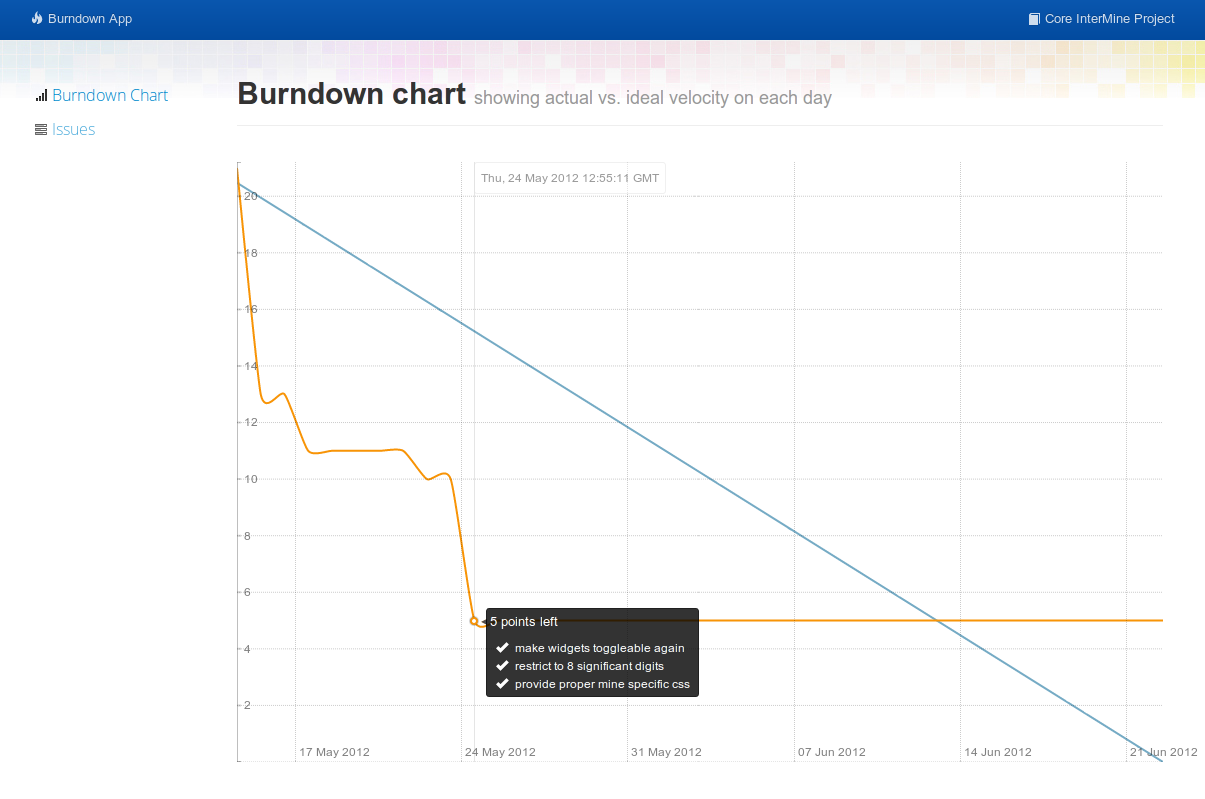
\includegraphics[width=0.98\textwidth, keepaspectratio=true]{githubburndownexample}
\caption{GitHub Burn-down application}
\label{githubburndownexample}
\end{figure}

\subsubsection*{HuBoard}
\emph{GitHub issues made awesome.} \footnote{\url{http://huboard.com/}} \\
HuBoard is a project management tool, which takes your GitHub issues and milestones and generates a Kanban\footnote{Kanban is a software development method with focus on Just-in-time delivery. Developers pick tasks from a queue. \url{http://www.kanbanblog.com/explained/index.html}} board built from the GitHub api. \\
This tool features the idea of scaffolding issues and milestones into something useful for a different context, although it is limited to issues and have no features for capturing experience and promoting reflection. 
\subsubsection*{Agile Bench}
Agile Bench integrates with GitHub so programmers do not have to duplicate comments between two systems\footnote{Agile Bench GitHub integration: \url{http://support.agilebench.com/entries/21307153-GitHub-Integration}}. Instead they can make a comment via GitHub(the code base) commits and this will push comments into the project management system. AgileBench supports these commit formats:
\begin{itemize}
\item \verb|[#story_id]| comment - i.e. "[\#5] Added documentation" - will add "Added documentation" to story \#5
\item \verb|[#story_id #story_id]| comment. i.e. "[\#5 \#6] Added even more documentation" - will add "Added documentation" to story \#5 and \#6
\item \verb|[Workflow State #story_id #story_id]| comment. i.e. "[In Progress \#5 \#6] Added even more documentation" - will add "Added even more documentation" to story \#5 and \#6 and move stories \#5 \& \#6 into the In Progress workflow state.
\end{itemize}
Agile Bench do not facilitate for experience collection in order to promote reflection.
\subsubsection*{AgileZen}
AgileZen also organizes work in a Kan-ban board, with user-stories\footnote{AgileZen: \url{http://www.agilezen.com}}. Zen features teams with users and different user-roles. It also allows artifacts like screen shots or specification documents to be attached to a story. It integrates with GitHub as a service hook\footnote{\url{https://help.github.com/articles/post-receive-hooks}}. In order for Zen to include your change sets from GitHub, you need to refer to the story ID in your commits using the format \#123 or zen-123. This further builds on the idea of using \#hash-tags to \textit{tag} relevant messages and identify them in your commits. 

\section{Discussion}
There are several tools that display data collected from VCS like GitHub as described in the previous section, although these tools display data in a different context and with a different goal. Where as we aim to display data for the purposes of connecting these data with experiences to trigger reflection, these tools display data for project management purposes or to gather research data(I.e. \emph{HackyStat}). Common for all the tools introduced in section \ref{subsec:gittools} are their tight connection with GitHub which allows for efficient data collection.

\subsubsection{HackyStat}
\emph{HackyStat} is very general, but aims at collecting usage statistics from software development teams or users. These data are used for reports which are stored for later use to facilitate \emph{Collective intelligence}. We used this for inspiration towards the notion of storing reflection notes for later use, both individually and collaboratively as a team as preparation before the retrospective session.   

\subsubsection{GitHub Burn-Down Chart}
The \emph{GitHub Burn-down} application is a small, yet informative application for development teams using scrum as their agile development process. The application creates a burn-down chart of the current GitHub-project milestone and displays all issues connected to it. The burn-down application has no direct connection to reflection and it's functionality were therefore not implemented, but was used for inspiration when designing the interaction between GitHub and the PeacefulBanana application. 

\subsubsection{HuBoard}
\emph{HuBoard} is similar to the GitHub burn-down application in the sense that it connects with GitHub and makes use of project milestones and issues that are present, in order to generate a KanBan board\footnote{Agile process for just-in-time(JIT) production}. This tailors the milestones and issues to be used in a better way, more suited for agile development methods. Similar to the GitHub burn-down application discussed above we looked at the integration with GitHub and used that for inspiration on how to best connect and collect data from GitHub through our own application. 
HuBoard also provided design related inspiration, as the tool is implemented with the \emph{Twitter Bootstrap} framework.

\subsubsection{Agile Bench}
\emph{Agile Bench} provided several ideas we wanted to bring to the PeacefulBanana application. Agile Bench uses \#-Hash-tags to annotate commits, much in the same way we intended with PeacefulBanana. Also, giving users the possibility to attach feelings and general comments to specific milestones or issues are definitely ideas we wanted to integrate in the application.

\subsubsection{AgileZen}
\emph{AgileZen} provided some ideas in the aspect of teams with users and giving the users different roles(i.e. manager or developer). AgileZen also uses \#hash-tags to annotate commits, which provided even more justification that hash-tags was a viable way of annotating commits.  